% \documentclass[border=0]{standalone}
\documentclass[a4paper]{article}
% \documentclass[aip]{revtex4-2}
%\documentclass[aip,reprint]{revtex4-2}
\usepackage[margin=1mm]{geometry}
\usepackage{graphicx}
\usepackage{float}
\usepackage{tikz}
\usetikzlibrary{patterns,patterns.meta}
\usepackage{ccicons}
\usepackage[hidelinks]{hyperref}
% \draft % marks overfull lines with a black rule on the right

\begin{document}
\thispagestyle{empty}
\begin{figure}
    \centering
    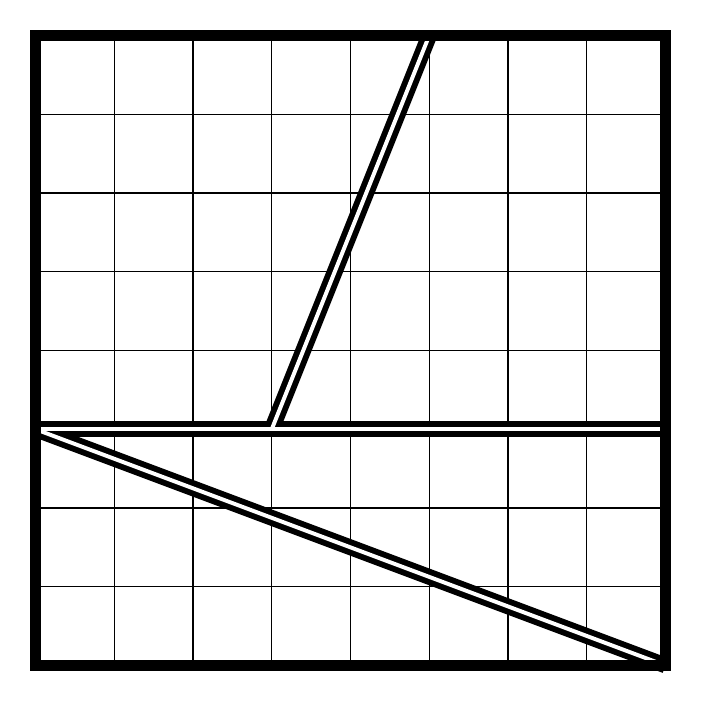
\begin{tikzpicture}
        \draw (0,0) grid (8,8);
        \draw[line width=2mm] (0,3) -- (8,3);
        \draw[line width=2mm] (0,3) -- (8,0);
        \draw[line width=2mm] (3,3) -- (5,8);
        \draw[line width=0.5mm,white] (0,3) -- (8,3);
        \draw[line width=0.5mm, white] (0,3) -- (8,0);
        \draw[line width=0.5mm, white] (3,3) -- (5,8);
        \draw[line width=1.5mm] (0,0) rectangle (8,8);
    \end{tikzpicture}
    
\end{figure}
\begin{figure}
    \centering
    
\begin{tikzpicture}
        \draw[->,line width=1mm] (0,0) -- (270:1);
        \end{tikzpicture}
\end{figure}
\begin{figure}
    \centering
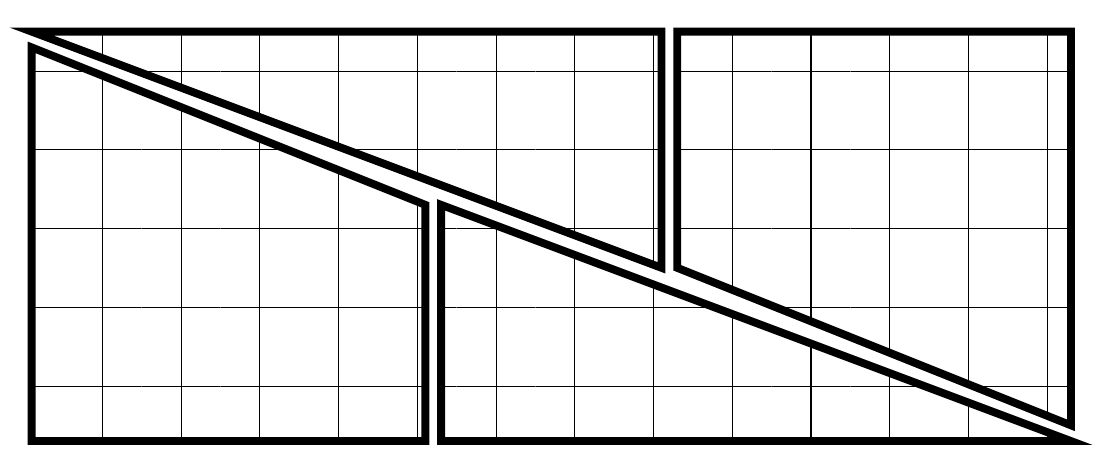
\begin{tikzpicture}
    % Draw the polygon
    \draw[line width=1mm] (0,0) -- (5,0) -- (5,3) -- (0,5) -- cycle;
    \draw[line width=1mm] (5.2,3) -- (5.2,0) --++ (0:8) -- cycle;
    \draw[line width=1mm] (0,5.2) --++ (0:8) --++ (270:3) -- cycle;
    \draw[line width=1mm] (13.2,0.2) --++ (90:5) --++ (180:5) --++ (270:3) -- cycle;
    % Add grid pattern
    \draw[pattern={Hatch[distance=1cm,xshift=0.3cm,yshift=0.1cm]}] (0,0) -- (5,0) -- (5,3) -- (0,5) -- cycle;
    \draw[pattern={Hatch[distance=1cm,xshift=0.3cm,yshift=0.1cm]}] (5.2,3) -- (5.2,0) --++ (0:8) -- cycle;
    \draw[pattern={Hatch[distance=1cm,xshift=0.3cm,yshift=0.1cm]}] (0,5.2) --++ (0:8) --++ (270:3) -- cycle;
    \draw[pattern={Hatch[distance=1cm,xshift=0.3cm,yshift=0.1cm]}] (13.2,0.2) --++ (90:5) --++ (180:5) --++ (270:3) -- cycle;\end{tikzpicture}
\end{figure}
% \begin{figure}
%     \begin{tikzpicture}
%         \draw (0,0) grid (13,13);
%         \draw[very thick] (0,5) -- (13,5);
%         \draw[very thick] (0,5) -- (13,0);
%         \draw[very thick] (5,5) -- (8,13);
%     \end{tikzpicture}
% \end{figure}
% \vfill
% \ccbyncsa
% \hfill \today, \href{https://dishajk@github.io}{dishajk@github.io}
\end{document}